%
% instructions for "compiling":
%   latex main (first pass, also generates .aux file for bibtex)
%   bibtex main (generates .bbl file with bibliography)
%   latex main (second pass, incorporates bibliography)
%   latex main (do this if you still get messages about labels
%      having changed or missing references)
% to generate/view/print postscript:
%   dvips -o main.ps main 
%   gv main.ps (to view)
%   lpr main.ps (to print, or print from "gv")
% to generate/view/print PDF:
%   dvips -Pcmz -Ppdf -j0 -G0 -o main.ps main
%   ps2pdf main.ps main.pdf
%   acroread main.pdf (to view/print)
%   
\documentclass[11pt]{report}

% miscellaneous packages
% FIX THIS -- can add to or change, but these are useful
\usepackage{amsmath}
\usepackage{graphicx}
\usepackage{moreverb}
\usepackage{url}

% double spacing
\usepackage{setspace}
\doublespacing

% hyphenation
\usepackage[english]{babel}
\selectlanguage{english}

% allow more figures on a page
\setcounter{topnumber}{10}
\setcounter{bottomnumber}{10}
\setcounter{totalnumber}{10}
\setcounter{dbltopnumber}{10}
\def\topfraction{1.0}
\def\bottomfraction{1.0}
\def\textfraction{0.0}
\def\dbltopfraction{1.0}

% margins
%\usepackage[letterpaper,top=2.0in,bottom=1.5in,left=1.5in,right=1.0in]
%	{geometry}
\usepackage[top=2.0in,bottom=1.5in,left=1.5in,right=1.0in]{geometry}

% set up to put page numbers in header
\usepackage{fancyhdr}
\pagestyle{fancy}
\lhead{}
\chead{}
\rhead{\rm\thepage}
\lfoot{}
\cfoot{}
\rfoot{}
\renewcommand{\headrulewidth}{0pt}
\renewcommand{\footrulewidth}{0pt}

% author, title, and date
% FIX THIS
\newcommand{\theAuthor}{Your Name Here}
% FIX THIS -- but be sure to leave in \par if title might exceed
%   one line -- otherwise space between lines will be wrong
\newcommand{\theTitle}{Your Title Goes Here
	(It Can Be Really Really Really Really Long)\par}
% FIX THIS
\newcommand{\theDate}{April 1, 2005}

% FIX THIS -- can put additional macro definitions here

%----------------------------------------------------------------------

\begin{document}

\pagenumbering{gobble}

%
% spacing could probably be improved
%

\begin{center}

\bigskip

\begin{Large}
\textbf{\theTitle}
\end{Large}

\bigskip

\begin{large}
\theAuthor
\end{large}

\bigskip
\bigskip

\textbf{Abstract}

\end{center}

\noindent
% FIX THIS --- your abstract goes here.
A nice abstract goes here.



\clearpage
%
% spacing could probably be improved
%
\begin{center}

\bigskip

\begin{Large}
\textbf{Acknowledgments}
\end{Large}

\bigskip

\end{center}

%FIX THIS --- thank your advisor, etc., here.
Some acknowledgments go here.



\clearpage
\begin{center}

\vfill

\textbf{\theTitle} %\\

\theAuthor \\

\vspace*{\baselineskip}

A departmental thesis submitted to the \\
Department of Computer Science at Trinity University \\
in partial fulfillment of the requirements for Graduation.\\
% with departmental honors. 

\vspace*{\baselineskip}

\theDate

\vfill

$\overline{\mbox{\rule{0in}{0.16in}Thesis Advisor~~~~~~~~~~~~~~~~~~~~~~~~~~}}$ 
\hfill
$\overline{\mbox{\rule{0in}{0.16in}Department Chair~~~~~~~~~~~~~~~~~~~~~~~~}}$ 

\vspace{1.0in}

$\overline{\mbox{\rule{0in}{0.16in}
~~~~~~~~Associate Vice President~~~~~~~~
}}$ \\
for \\
Academic Affairs

\vfill

\hfill
\hfill
\hfill

\begin{tiny}
%This work is licensed under the Creative Commons Attribution-NonCommercial-NoDerivs License.  To view a copy of this license, visit <http://creativecommons.org/licenses/by-nc-nd/2.0/> or send a letter to Creative Commons, 559 Nathan Abbott Way, Stanford, California 94305, USA.
This work is licensed under the Creative Commons Attribution-NonCommercial-NoDerivs License.  To view a copy of this license, visit \textless http://creativecommons.org/licenses/by-nc-nd/2.0/\textgreater or send a letter to Creative Commons, 559 Nathan Abbott Way, Stanford, California 94305, USA.
\end{tiny}


\end{center}


\clearpage
%
% spacing could probably be improved
%

\begin{center}

\vfill

\begin{Huge}
\textbf{\theTitle}
\end{Huge}

\bigskip \bigskip \bigskip

\begin{huge}
\theAuthor
\end{huge}

\vfill

\end{center}


\tableofcontents
\listoftables
\listoffigures

\clearpage
\pagenumbering{arabic}

% FIX THIS -- one file per chapter is good but not required
%
% FIX THIS -- remove/change, just some examples of things
%
\chapter{Example chapter}

Example chapter, with apologies to Alex Kolliopoulos,
from whose thesis the examples of math and tables were
borrowed.

\section{Examples of figures and tables}
\label{section:example-figtbl}

This section contains some words, plus
Figure~\ref{fig:xor} and 
Table~\ref{table:treepurpose}.

words, words, words, words,
words, words, words, words,
words, words, words, words,
words, words, words, words,
words, words, words, words,
words, words, words, words,
words, words, words, words,
words, words, words, words,

\begin{figure}[hbtp]
\begin{center}
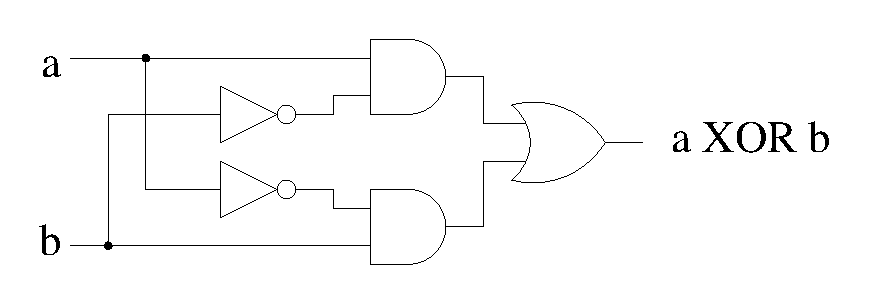
\includegraphics[width=0.5\textwidth]{xor}
\end{center}
\caption{An example figure.}
\label{fig:xor}
\end{figure}

words, words, words, words,
words, words, words, words,
words, words, words, words,
words, words, words, words,
words, words, words, words,
words, words, words, words,
words, words, words, words,
words, words, words, words,

\begin{table}[hbtp]
\begin{tabular}{|l|l|}
\hline 
\textbf{Trial 1} & Expanding a node to select a child\\
\hline
\textbf{Trial 3} & Selecting a node near the middle of a long, linear list\\
\hline
\textbf{Trial 4} & Selecting a node near the top of a long, linear list\\
\hline
\textbf{Trial 5} & Selecting a node near the bottom of a long, linear list\\
\hline
\textbf{Trial 6} & Scrolling and expanding folders in a large tree\\
\hline
\textbf{Trial 7} & Finding a node deep and near the bottom in a large tree\\
\hline
\textbf{Trial 8} & Finding a node near the top of a large tree\\
\hline
\end{tabular}
\caption{Purposes of each experimental trial.}
\label{table:treepurpose}
\end{table}
\section{Examples of math}
\label{section:example-math}

This section contains some math.
First, here's a set of equations.

\begin{eqnarray*}
y_p	&	=	&	\frac{y}{\sqrt{y^2+a^2}}, \\
y_p^2	&	=	&	\frac{y^2}{y^2+a^2}, \\
y_p^2	&	=	&	\frac{y^2+a^2-a^2}{y^2+a^2}, \\
y_p^2	&	=	&	1-\frac{a^2}{y^2+a^2}, \\
y_p^2-1	&	=	&	-\frac{a^2}{y^2+a^2}, \\
1-y_p^2	&	=	&	\frac{a^2}{y^2+a^2}.
\end{eqnarray*}

words, words, words, words,
words, words, words, words,
words, words, words, words,
words, words, words, words,
words, words, words, words,
words, words, words, words,
words, words, words, words,
words, words, words, words,

Now here's a numbered equation.

\begin{equation}
0 = 0 \label{eqn:example}
\end{equation}

\section{Examples of references}

% the "~" makes a no-line-breaks space
Section~\ref{section:example-figtbl} contains 
Figure~\ref{fig:xor} and
Table~\ref{table:treepurpose}.
Section~\ref{section:example-math} contains
Equation~(\ref{eqn:example}).
The sample bibliography file contains references to
a book \cite{gof-book} and a Web site \cite{MPI2}, plus some
other things.
% put in bibliography even though not referenced
\nocite{Dijkstra80}
\nocite{plop03-paper}


% FIX THIS -- refs.bib is the bibtex file
\bibliography{refs}
\bibliographystyle{plain}

\appendix
% FIX THIS
\chapter{A Partial J Lexer Written in Scala}
\label{jlex}

\begin{singlespacing} 
\begin{small}
\verbatimtabinput{JLexer.scala}
\end{small}
\end{singlespacing}


\end{document}
